\documentclass[12pt]{article}
\usepackage[english]{babel}
\usepackage[utf8]{inputenc} 
\usepackage[T1]{fontenc}
\usepackage{graphicx}
\usepackage{amsmath}
\usepackage{wrapfig}
\usepackage{enumerate}
\usepackage[top=1in, bottom=1.25in, left=1.1in, right=1.1in]{geometry}
\usepackage[dvipsnames]{xcolor}
\usepackage{subcaption}

\begin{document}

\begin{titlepage}

\newcommand{\HRule}{\rule{\linewidth}{0.5mm}} 

\center 

\textsc{\LARGE Universidad de Sonora}\\[1.5cm]
\textsc{\Large Licenciatura en Física}\\[0.5cm]
\textsc{\large Física Computacional I}\\[0.5cm]

\HRule \\[0.4cm]
{\huge \bfseries Actividad 9 - Sistema de Algebra Computacional Maxima}\\[0.4cm] 
\HRule \\[1.5cm]

\begin{minipage}{0.4\textwidth}
\begin{flushleft} \large
\emph{Alumno:}\\
José Gabriel Navarro I.
\end{flushleft}
\end{minipage}
~
\begin{minipage}{0.4\textwidth}
\begin{flushright} \large
\emph{Profesor:} \\
Carlos Lizarraga Celaya
\end{flushright}
\end{minipage}\\[2cm]

28 de Abril de 2018


\includegraphics[width=0.4\textwidth]{logo.png}\\
 
\vfill

\end{titlepage}

\section{Introducción}
En el presente reporte se presenta la Actividad 9 para la clase de Física Computacional I, en donde se utiliza el nuevo sistema de Álgebra Computacional "Maxima". Un sistema algebraico computacional es un programa de ordenador  que facilita el cálculo simbólico. La principal diferencia entre este y una calculadora normal es el poder para trabajar con ecuaciones y fórmulas simbólicamente, en lugar de numéricamente, además de que estos sistemas nos permite automatizar manipulaciones tediosas o difíciles, como por ejemplo, alguna integral, o una multiplicación de matrices. \\

En este reporte se presenta un pequeño manual de las funciones principales que tiene Maxima, el uso de sus variables, como procesa la información, almacenamiento de variables, entre otras cosas. También se incluye distintas aplicaciones que puede tener este programa en la solución de otros problemas que involucran materias que actualmente se están cursando, como lo es Calculo, o materias que ya se han cursado como Geometría y Álgebra Lineal. 

\section{Características principales}
A continuación se presenta un resumen de las características principales del funcionamiento de Maxima. Es importante conocer como funciona y lee variables este programa, ya que al realizar cálculos extensivos, un error de sintaxis podría causar una cadena de errores.

\subsection{Entrada y salida de información}
Cuando se inicia una nueva sesión de Maxima, a la izquierda de la ventana aparecerá un una etiqueta como la siguiente: (\%i1). Esto indica que es el "input 1", y al dar Shift+Enter, esta entrada sera simplificada y será vinculada a una variable interna de la etiqueta correspondiente. El resultado de la variable (\%i1), será mostrada en pantalla pero esta vez con la etiqueta (\%o1), de "output 1". Al introducir una nueva linea, la etiqueta ira aumentando, es decir: (\%i2), (\%i3), etc. 

\begin{figure}[h!]
    \centering
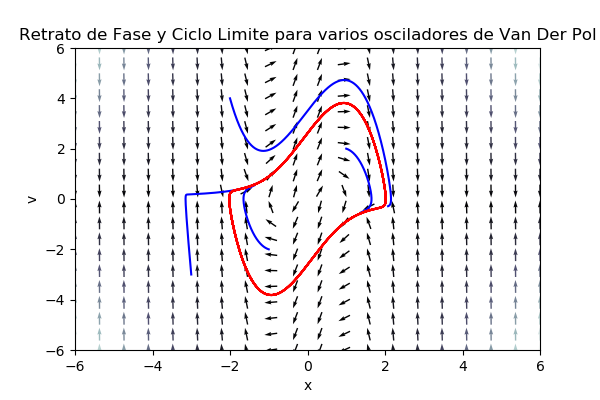
\includegraphics[width=2in]{Im1.png}
\end{figure}

Como se puede observar, para realizar operaciones, se realiza con la sintaxis que se presenta mas comúnmente en libros de texto o otros lenguajes de programación, como Fortran o C. La salida 2 no se muestra en pantalla ya que el valor del logaritmo es irracional, entonces no puede ser representado por un numero finito de dígitos. Para saber la descripción completa de un comando, podemos utilizar el comando \textit{describe}, o el signo "?" antes del comando:

\begin{figure}[h!]
    \centering
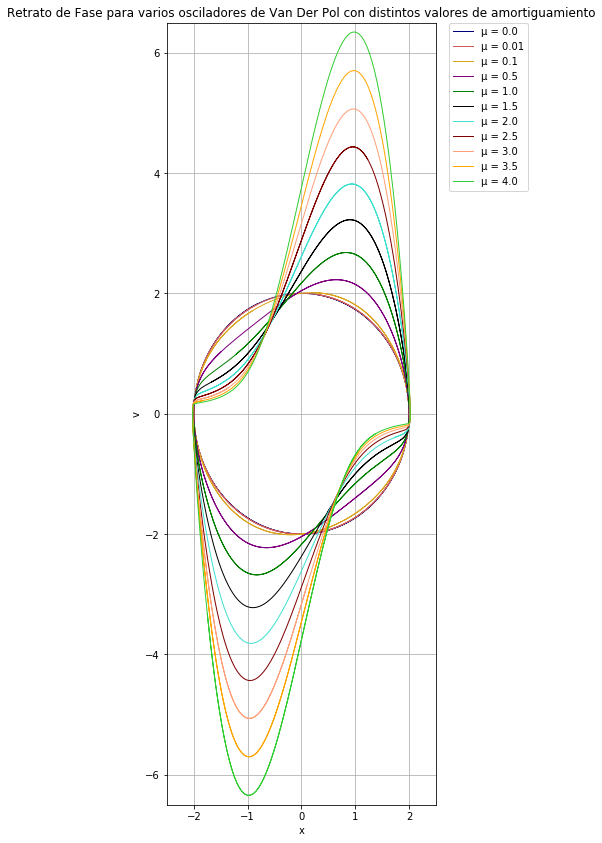
\includegraphics[width=5in]{Im2.png}
\end{figure}

\subsection{Números}
Maxima acepta números reales e imaginarios. Los números reales pueden ser tanto enteros, como racionales, fraccionarios, o de punto flotante. Sin embargo, como se pudo notar en la primera imagen, al calcular un numero irracional, este no es mostrado en pantalla, e incluso si se multiplica por un numero entero, este sigue sin mostrarse en pantalla. \\

Para hacer que estos puedan ser mostrados en pantalla, podemos utilizar la función \textit{float}, que permite mostrar en pantalla el valor numérico real. Pero una cosa al considerar es que la precisión sencilla tal vez no muestre el valor exacto, o nos pueda dar operaciones simples en un formato innecesario: 

\begin{figure}[h!]
    \centering
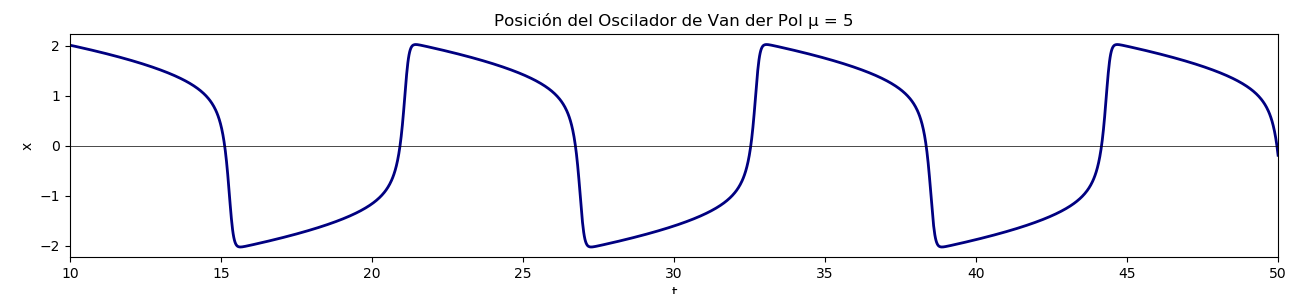
\includegraphics[width=2.5in]{Im3.png}
\end{figure}

Si se desea mas precisión, podemos indicarlo mediante el formato \textit{Big Float}, el cual muestra mas dígitos basado en el valor de la variable de \textbf{fpprec}. Por ejemplo, si deseamos mas dígitos para la operación antes presentada se realiza lo siguiente:

\begin{figure}[h!]
    \centering
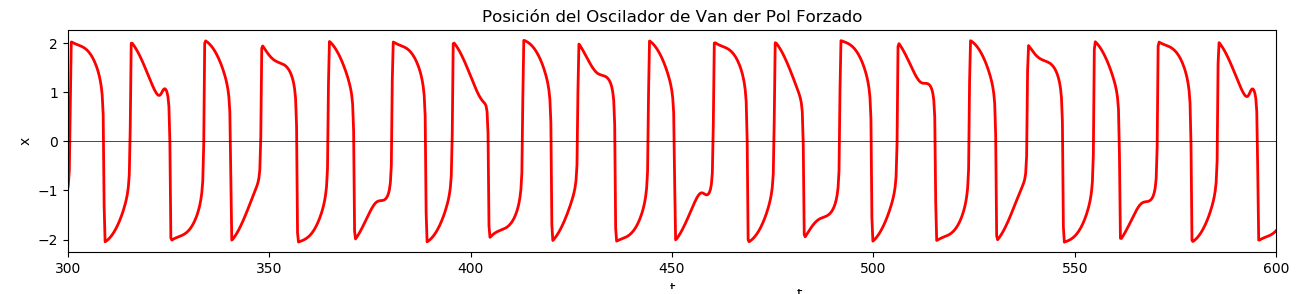
\includegraphics[width=4in]{Im4.png}
\end{figure}

\pagebreak

\subsection{Variables}
Se le puede asignar a un numero o operación un nombre. Para darle dicho nombre, se utiliza el símbolo ":", y no el signo igual (ese esta reservado para las ecuaciones). El nombre de las variables puede ser cualquier combinación de letras, números y de los símbolos \% y \_, pero no puede comenzar con un número:

\begin{figure}[h!]
    \centering
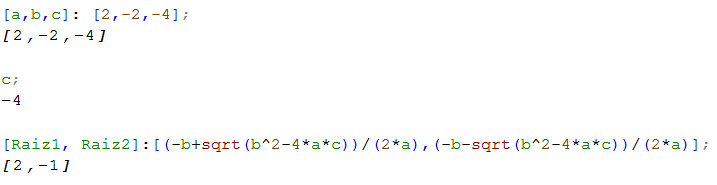
\includegraphics[width=4in]{Im5.png}
\end{figure}

Se puede asignar una ecuación a una variable, solamente indicando las variables de la ecuación. Si se quiere sustituir los valores a la ecuación, se utiliza el comando \textit{subst}, seguido por los valores de las variables y el nombre de la variable en la que se va a reemplazar:

\begin{figure}[h!]
    \centering
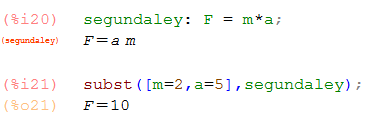
\includegraphics[width=4in]{Im6.png}
\end{figure}

\subsection{Listas}
Una variable también puede ser vinculada a una lista de datos, los cuales se ponen dentro de los corchetes separados por una coma y pueden ser utilizados en operaciones:

\begin{figure}[h!]
    \centering
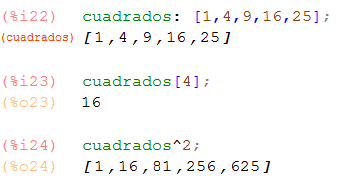
\includegraphics[width=4in]{Im7.png}
\end{figure}

\pagebreak

También pueden crearse listas a partir contadores con el comando \textit{makelist}, en donde el primer comando muestra la operación que se va a realizar, la variable, el inicio y el final (si se da un quinto parámetro, se toma como el incremento):

\begin{figure}[h!]
    \centering
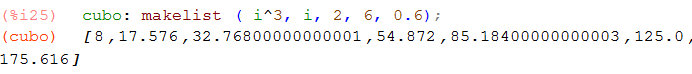
\includegraphics[width=5in]{Im8.png}
\end{figure}

\subsection{Constantes}
Existen algunas constantes ya predefinidas por Maxima. Estas variables son llamadas mediante el símbolo "\%". Unos ejemplos de ellos son el valor de $\pi$, el numero de Euler, y el numero imaginario $i$: 

\begin{figure}[h!]
    \centering
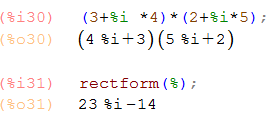
\includegraphics[width=3in]{Im9.png}
\end{figure}

Si se desea operar con números imaginarios y ver su forma rectangular se usa el comando \textit{rectform}.

\section{Álgebra}
Las expresiones pueden incluir operaciones matemáticas con variables aun no definidas, para posteriormente realizar otro tipo de operaciones con ellas. Si estas son igualadas a otra expresión, se puede encontrar las raíces de la ecuación, tal como se muestra en la siguiente imagen:

\begin{figure}[h!]
    \centering
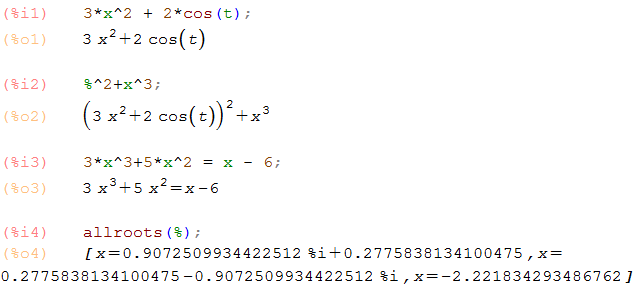
\includegraphics[width=4.5in]{Al1.png}
\end{figure}

\pagebreak

Es posible también expandir polinomios de distintos grados utilizando la función \textit{expand} y posteriormente reemplazar los valores que deseemos con alguna expresión o valor, utilizando la función \textit{subst}. Esto facilita mucho el hacer integrales triples o dobles para expresiones grandes, como mas adelante vamos a ver:

\begin{figure}[h!]
    \centering
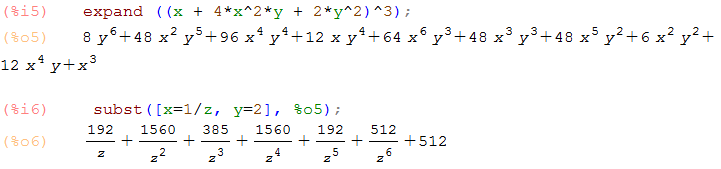
\includegraphics[width=4.5in]{Al2.png}
\end{figure}

\section{Gráficas en 2D y 3D}
El comando \textit{plot2d} permite realizar graficas de una o varias funciones de una variable. Por ejemplo, para una función polinomial de una variable, se puede obtener una gráfica como la siguiente:

\begin{figure}[h!]
    \centering
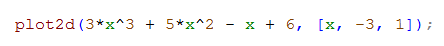
\includegraphics[width=4.5in]{Graf2.png}
\end{figure}
\begin{figure}[h!]
    \centering
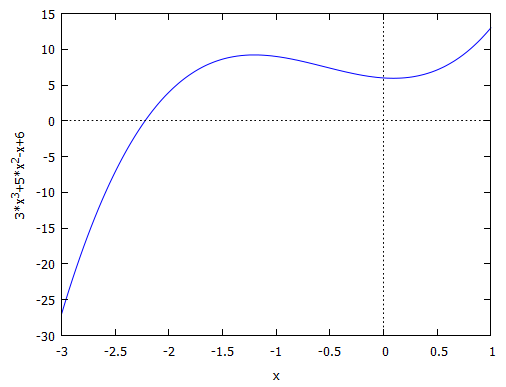
\includegraphics[width=4.5in]{Graf1.png}
\end{figure}

\pagebreak

O si se desea realizar una gráfica con distintas funciones, una sobre la otra, solamente se ponen dentro de una lista con sus limites: 

\begin{figure}[h!]
    \centering
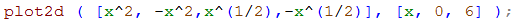
\includegraphics[width=4.5in]{Graf4.png}
\end{figure}
\begin{figure}[h!]
    \centering
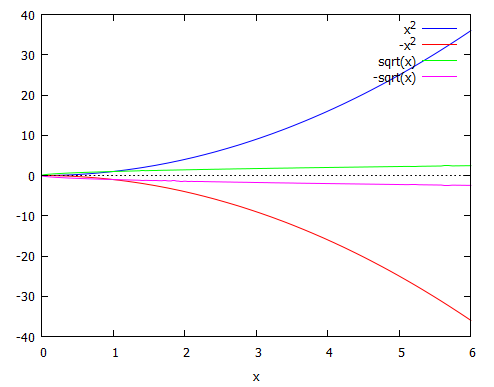
\includegraphics[width=4.5in]{Graf3.png}
\end{figure}

Es posible también realizar graficas en 3D, simplemente utilizando la función \textit{plot3d}, en donde se coloca la función, y los parámetros de las dos variables independientes:

\begin{figure}[h!]
    \centering
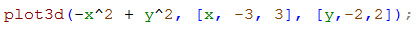
\includegraphics[width=4in]{Graf6.png}
\end{figure}
\begin{figure}[h!]
    \centering
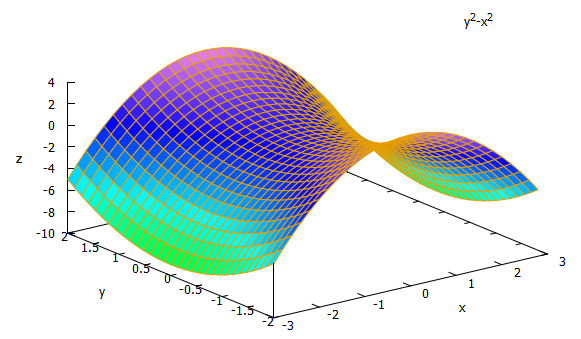
\includegraphics[width=4in]{Graf5.png}
\end{figure}

\subsection{Parametrización de curvas y superficies}
Además de poder realizar graficas en 2D y 3D a partir de funciones de variables dependientes e independientes, es posible también realizar parametrizaciones de curvas y superficies utilizando las mismas funciones anteriormente utilizadas. La diferencia esta en que ahora se debe indicar dentro de la función, el parametro \textit{parametric}. En 2D, un ejemplo es:

\begin{figure}[h!]
    \centering
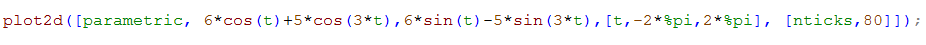
\includegraphics[width=5in]{Graf8.png}
\end{figure}
\begin{figure}[h!]
    \centering
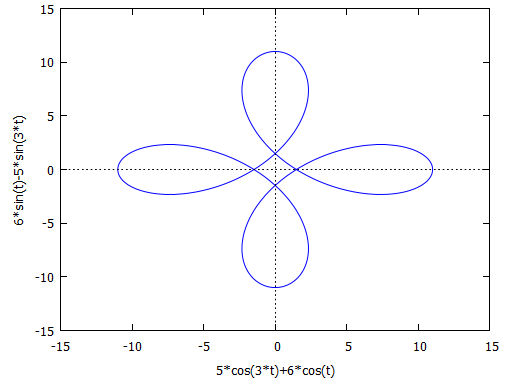
\includegraphics[width=3.5in]{Graf7.png}
\end{figure}

Y en 3D, se pueden parametrizar superficies, como toroides:

\begin{figure}[h!]
    \centering
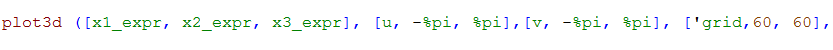
\includegraphics[width=5in]{Graf10.png}
\end{figure}
\begin{figure}[h!]
    \centering
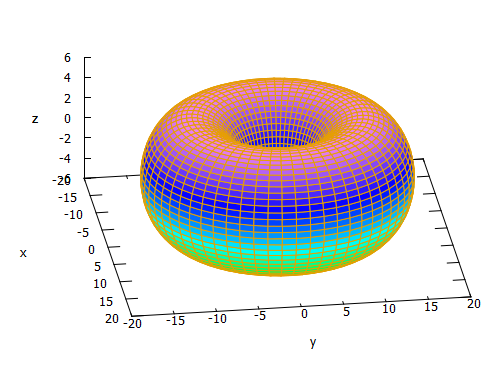
\includegraphics[width=3in]{Graf9.png}
\end{figure}

\section{Álgebra Lineal}
El uso de matrices y sus distintas operaciones se utilizan mucho en varias áreas de la ciencia, por lo cual es de mucha ayuda saber como se definen y se operan. Para definir una matriz, se le asigna a una variable, y se utiliza la función \textit{matrix}, seguido por los componentes de cada vector. Es posible también observar una columna o renglón en especifico:

\begin{figure}[h!]
    \centering
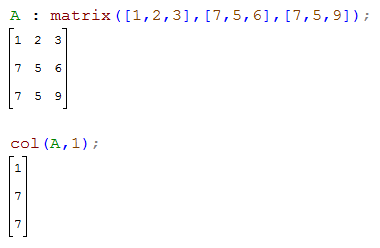
\includegraphics[width=4in]{Lin1.png}
\end{figure}

Incluso se puede realizar operaciones como sacar el determinante y la matriz inversa:

\begin{figure}[h!]
    \centering
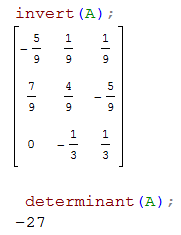
\includegraphics[width=2.5in]{Lin2.png}
\end{figure}

\pagebreak

También se pueden realizar las operaciones normales entre matrices, como suma, resta, multiplicación, división etc. Entonces, con estas herramientas se nos puede facilitar mucho solucionar sistemas de ecuaciones complejos, como los que se pueden dar en circuitos eléctricos. Por ejemplo, con el sistema que sale del análisis de un circuito realizado en la clase de Electromagnetismo se obtuvo:

\centerline{$i_1 -i_3 -i_5 = 0$}
\centerline{$i_1 +i_2 -i_3 -i_5 = 0$}
\centerline{$-6i_2 -15i_4 = -36$}
\centerline{$-6i_2 + 4i_3 -5i_5 = -20$}
\centerline{$-6i_1 - 4i_3 = 6$}
$    $

Y recordando como se resuelven los sistemas de ecuaciones mediante el uso de la matriz inversa: \\

\centerline{$x = A^{-1} b$}
$     $

Tenemos que:

\begin{figure}[h!]
    \centering
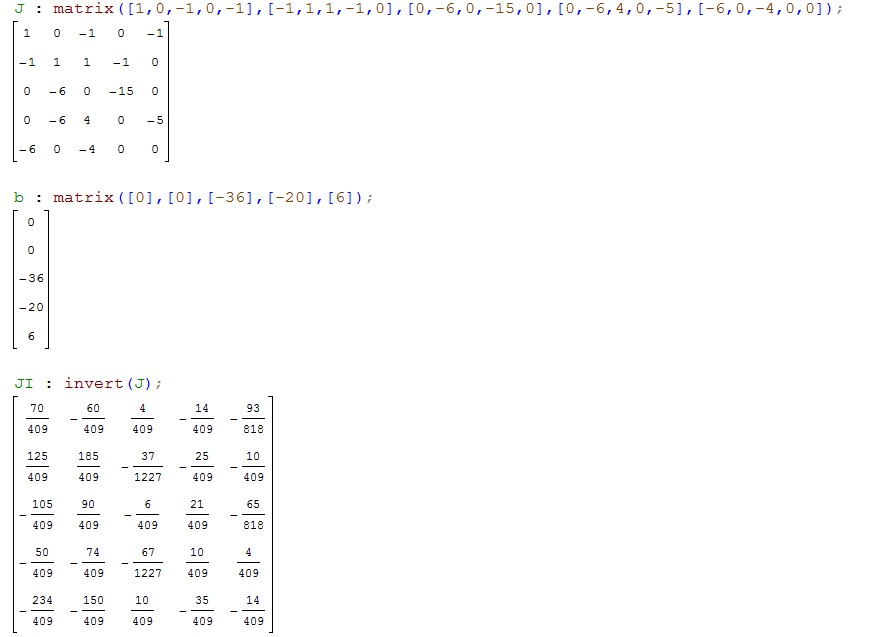
\includegraphics[width=6in]{Lin3.png}
\end{figure}

En donde las soluciones es la multiplicación entre la matriz b y JI, en donde se obtuvo los resultados que se obtuvieron en clase:

\begin{figure}[h!]
    \centering
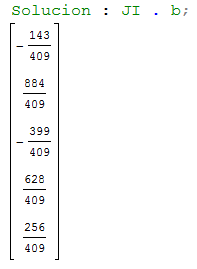
\includegraphics[width=2.5in]{Lin4.png}
\end{figure}

\section{Cálculo}
Maxima tambien es capaz de desarrollar derivadas e integrales, ya sea definidas o no. Para derivar se utiliza el comando \textit{diff}, y para integrar se utiliza el comando \textit{integrate} por ejemplo:

\begin{figure}[h!]
    \centering
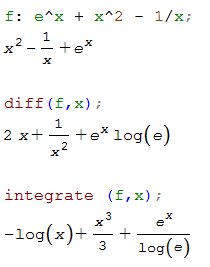
\includegraphics[width=2.5in]{Cal1.png}
\end{figure}

\pagebreak

Como se menciono anteriormente, también se pueden evaluar las funciones para ciertos valores, o se pueden integrar con limites:

\begin{figure}[h!]
    \centering
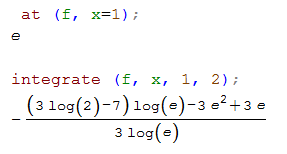
\includegraphics[width=2.5in]{Cal2.png}
\end{figure}

Lo cual resulta algo muy útil, ya que en nuestro curso de Calculo Vectorial, se utilizan mucho las integrales dobles y triples para cálculos de volúmenes, y es muy difícil comprobar con paginas de internet, ya que a veces no procesa bien los datos. Por ejemplo: \\

\noindent \textbf{Determine el volumen del solido limitado por el paraboloide eliptico $z= 1 +(x-1)^2 + 4y^2$, los planos $x=3, y=2$ y los planos coordenados.} \\

El volumen que se calculo en clases fue de $44 u^3$, Maxima nos permite saber si este resultado es correcto. El volumen que se quiere encontrar es el siguiente:

\begin{figure}[h!]
    \centering
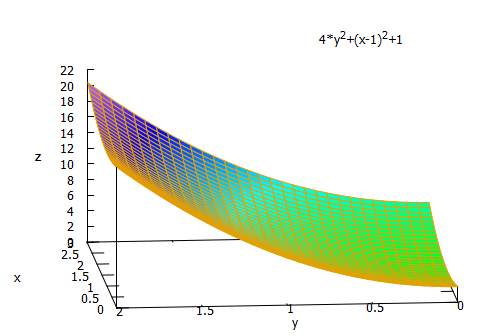
\includegraphics[width=4in]{Cal3.png}
\end{figure}

Y al realizar la integral, se obtiene que el valor del volumen es el mismo que se obtuvo en clase:

\begin{figure}[h!]
    \centering
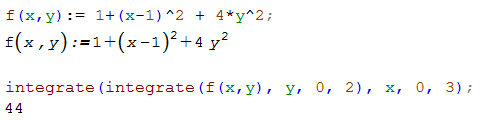
\includegraphics[width=3in]{Cal4.png}
\end{figure}

\section{Conclusión}
 Maxima y todos los Sistemas Algebraicos Computacionales, son una gran herramienta que facilita mucho los cálculos matemáticos que nosotros a mano nos podemos tardar casi horas. Me parece fascinante todo el poder que tiene este programa para realizar graficas, integrales, derivadas, operaciones de matrices, expansiones y muchas mas cosas que no se mencionaron con gran facilidad y en un tiempo casi inmediato. \\
 
Es muy importante aprender el uso y manejo de este programa, por lo cual, el realizar este manual fue de gran ayuda, ya que no solo se investigo como funciona en si el programa (desde lectura de datos hasta variables), si no que también se aprendió a manejar varias herramientas para su uso en nuestras clases. 

\section{Bibliografía empleada}
\begin{itemize}
    \item Sistema Algebraico Computacional. (2018). Recuperado de: www.ecured.cu/Sistema \\ \_Algebr\%C3\%aico\_Computacional
    \item Maxima Tutorial. (7 de Marzo de 2018). Recuperado de: def.fe.up.pt/dynamics \\/maxima\_tutorial.html
    \item Gráficos usando Maxima básico. (Agosto 2011). Recuperado de: webs.um.es/mira/maxima/ \\ GraficosMaxima.html
    \item Maxima by Example. (30 de Marzo de 2016). Recuperado de: web.csulb.edu/\~\\woollett/mbe5matrix.pdf
    \item Multivariable Calculus with Maxima. (1 de Diciembre de 2009). Recuperado de: gkerns.people.ysu.edu/maxima/maximaintro/maximaintro.pdf
\end{itemize}

\section{Apéndice}
\noindent\textbf {1. ¿Cuál fue tu primera impresión de wxmaxima?} \\

Me gusto mucho, como mencione anteriormente, me parece increíble el poder que tiene este programa para poder realizar tantos cálculos en tan poco tiempo y no solo eso, si no que también es de licencia gratuita. \\

\noindent\textbf {2. ¿Crees que esta herramienta puede ser útil en otros de tus cursos?} \\

Durante el reporte se habla acerca de como las herramientas tratadas pueden ser usadas en varias asignaturas, e incluso se resuelven algunos problemas de estas mismas, como lo fue el caso del circuito eléctrico y el volumen de la figura indicada, así que si. \\

\noindent\textbf {3. ¿Qué se te dificultó mas en esta actividad?} \\

La verdad nada, la instalación del programa fue facil y rápida y hay suficiente información en internet para poder realizar la actividad. \\

\noindent\textbf {4. ¿Se te hizo compleja esta actividad? ¿Cómo la mejorarías? } \\

No se me hizo compleja y no cambiaría nada. Me pareció una muy buena práctica. 
\end{document}